%
%  Vorlage/Template fuer #Proseminar
%
%  Created by Claudia Pittel und Yunus Erdemir in 2018, updated in 2021.
%  Copyright (c) 2021 . All rights reserved.
%
\documentclass[12pt,toc=bib,toc=listof]{scrreprt}
\usepackage[ngerman]{babel} 
\usepackage[utf8]{inputenc}
\usepackage[T1]{fontenc}
% Standardschriftart Latin Modern
\usepackage[scaled]{helvet}
\renewcommand\familydefault{\sfdefault}
% Arial, so in etwa
%\usepackage{newtxmath,newtxtext}
%Times New Roman, so in etwa
% Zitate durchgehend nummerieren
\usepackage{chngcntr}
\counterwithout{footnote}{chapter}
%Zeilenabstand
\usepackage{setspace}
\linespread{1.3}

% DIN-A-4, Ränder (oben, links, rechts, unten), Abstand Kopfzeile und Text
\usepackage{geometry}
\geometry{a4paper, top=25mm, left=30mm, right=20mm, bottom=25mm, headsep=12mm}

\usepackage[backend=bibtex, style=authortitle-ibid, url=false, isbn=false, doi=false]{biblatex}
\addbibresource{literature.bib}

\usepackage{hyperref}
\hypersetup{
  ,colorlinks=true
  ,linkcolor=blue
  ,citecolor=blue
  ,filecolor=blue
  ,urlcolor=blue
  }

%%%%%%%%%%%%%%%%%%%%%%%%%%%%%%%%%%%%% % (fold)
% Vom Studierenden zu aendernde Werte
\newcommand{\topic}{XaaS - Anything as a Service}

\newcommand{\studentnameA}{Suphi Pembe}
\newcommand{\studentidA}{207617}
\newcommand{\studentpartA}{SEITEN oder KAPITEL VON BIS 1}

\newcommand{\studentnameB}{Andreas Würzer}
\newcommand{\studentidB}{207258}
\newcommand{\studentpartB}{SEITEN oder KAPITEL VON BIS 2}

\newcommand{\studentnameC}{Christian Nguyen}
\newcommand{\studentidC}{207613}
\newcommand{\studentpartC}{SEITEN oder KAPITEL VON BIS 3}

\newcommand{\semester}{Sommersemester 2022}
%
%%%%%%%%%%%%%%%%%%%%%%%%%%%%%%%%%%%%% % (end)

\usepackage{ifpdf}
\ifpdf
\usepackage[pdftex]{graphicx}
\else
\usepackage{graphicx}
\fi

\usepackage[headsepline,footsepline]{scrlayer-scrpage}
\pagestyle{scrheadings}
\clearpairofpagestyles
\ihead{Proseminar: \topic}
\ofoot{Seite \pagemark}
\renewcommand*{\chapterpagestyle}{scrheadings}
\renewcommand*{\chapterheadstartvskip}{}

% Logo
\titlehead{\flushright
\includegraphics[scale=0.5]{HHN_Logo_D_oS_RGB_300.png}}
\subject{Proseminar (282136)}
\title{\topic}
\author{\studentnameA { ({\studentidA)}}, \\ \studentnameB { ({\studentidB)}}, \\ \studentnameC { ({\studentidC)}} }
\date {\semester}
%% Datum nie auf einen festen Wert setzen
\publishers{Vorgelegt bei Claudia Pittel}

%\pagestyle{headings}

% Zähler für Römische Nummerierung
\newcounter{savepage}

\begin{document}
\pagenumbering{roman} 
\selectlanguage{ngerman}
\sffamily
% serifenlose Schriftfamilie
\maketitle

\addchap{Management Summary} % (fold)
\label{sec:management_summary}

%Hier sollte ziemlich genau bzw. maximal 1 Seite Text stehen (ziemlich genau  bedeutet, man sollte so nah wie möglich an 1 Seite herankommen).

% chapter management_summary (end)

\tableofcontents

\addchap{Abkürzungsverzeichnis} % (fold)
\label{sec:abkuerzungsverzeichnis}

\begin{description}
\item[GPU] Graphics-Processing-Unit oder Grafikkarte
\item[HPC] High-Performance-Computing
\item[RAID] redundant array of independent disk
\end{description}

% chapter abkuerzungsverzeichnis (end)

\listoffigures
%\listoftables

% \onehalfspacing

\newpage
% Zähler speichern
\setcounter{savepage}{\arabic{page}}
\pagenumbering{arabic}

\chapter{Einleitung} % (fold)
\label{sec:einleitung}

%Einleitungstext mit Motivation, Ziel der Arbeit (d.h. Erläuterung der Forschungsfrage) und Beschreibung der Vorgehensweise bzw. Aufbau der Arbeit\footcite [vgl.] [S. 38]{Th17}

\section{Motivation} % (fold)
\label{sec:motivation}
%%%% Version 1 von Suphi %%%%%%%%
Durch den aktuell anhaltende Halbleitermangel besteht ein Engpass an Ressourcen von dem die meisten Wirtschaftszweige betroffen sind.
Einer dieser Wirtschaftszweige ist die Produktion von GPUs (graphics processing unit). Diese werden für diverse Prozesse in Computern verwendet, im betrieblichen wie auch im privaten Bereich.
Primär in dieser Arbeit werden die Bereiche High-Performance-Computing (HPC) und Gaming betrachtet.
Beide diese Bereiche benötigen GPU-Rechenleistung, welche konventionell von einer lokal verbauten GPU zur Verfügung gestellt wird. 
Als langfristige Lösung soll analysiert werden ob es möglich ist durch zentrale Services, welche GPU as a Service anbieten. 
Durch die zentralen Ressourcenteilung wird dem Mangel entgegengewirkt durch die Schaffung einer Alternative für den Bedarf.

% section motivation (end)

\section{Ziel der Arbeit} % (fold)
\label{sec:ziel_der_arbeit}

Das Ziel dieser Arbeit ist es den Markt um Cloud-Services zu verstehen, wie auch Potentiale und Gefahren 
dabei für die Zukunft in Betracht zu ziehen. Dabei wird ein Augenmerk auf Einsatzgebiete, welche 
vorallem GPU Leistung benötigen, gelegt.
Zunächst sollen die Begriffe Anything as a Service und Cloud Computing definiert werden. 
Dabei wird der Zusammenhang erläutert, wie auch die Unterschiede der Begriffe aufgezeigt.
Anschließend wird die aktuelle Knappheit von Grafikkarten analysiert und Gründe aufgezeigt.
In Beziehung mit der Knappheit sollen die Gaming as a Service und GPU as a Service, als Teil von Cloud Computing, 
betrachtet werden, da diese sehr von der Verfügbarkeit von GPUs abhängig sind.\\
Dabei soll durch die Möglichkeiten von Anything as a Service eine zentrale Ressourcenteilung an GPU Leistung 
geschaffen werden, um eine Alternative zu schaffen die benötigte GPU Leistung aus der Cloud zu beziehen.
Dabei sollen auch Zukunftsperspektiven aufgezeigt werden, um den zukünftigen Nutzen besser einschätzen zu können.\\
\\In Anbetracht dieses Ziels wollen wir folgende Forschungsfrage beantworten: "Wie können Angebote im Bereich Cloud Computing eine Alternative zum Kauf eines eigenen
Computers werden?"

% section vorgehensweise (end)
% chapter einleitung (end)

\chapter{Anything as a Service - Cloud Computing} % (fold)
\label{sec:Anything as a Service und Cloud Computing}

%Zwischen den Gliederungspunkten sollten jeweils kurze Überleitungssätze stehen, damit man weiß, um was es inhaltlich in den folgenden Unterkapiteln geht.\footcite [Vgl.] []{GPL}

% chapter ersteskapitel (end)

\section{Definition} % (fold)
\label{sec:Definition}

%Bei den Gliederungspunkten immer auf eine Ausgewogenheit achten, damit eine gleichmäßige Gliederung gefördert werden kann. Sofern Abbildungen (wie Abbildung 1: Beispielbild) verwendet werden, müssen diese auch inhaltlich im Text erwähnt und erläutert werden, sowie ein Abbildungsverzeichnis erstellt werden.\footcite [Vgl.] [] {hhnwin}
Everything/Anything as a Service: Oberbegriff für eine Kategorie an Services, die meist mit
 Cloud Computing oder Remote Acces in Verbindung stehen. Unternehmensinterne Dienste Ressourcen sollen anderen Akteuren in einem
 Dienstleistungsökosystem zur Verfügung gestellt werden. 
 Der Service steht hier klar im Vordergrund, zur Umsetzung kommen Technologien, wie beispielsweise: Blockchain, Machine Learning, 
 Distributed Ledger oder Cloud-Computing, zum Einsatz. In dieser Arbeit wird der Fokus auf das Cloud Computing gelegt. (Krcmar)
 \\ \\
 Cloud Computing: Bei Cloud Computing handelt es sich um die Bereitstellung von IT-Dienstleistungen, wie 
Speicherplatz, Rechenleistung, Datenbanken, über die Cloud, also das Internet. 
Die zur Verfügung stehenden Ressourcen sind dabei skalierbar, können also an den tatsächlichen Bedarf angepasst werden. Die, für Cloud Computing, gängigen Servicemodelle werden
in Kapitel 2.2 genauer behandelt. (Krcmar)
\\ \\
Die essenziellen Features/Eigenschaften einer Cloud Computing Umgebung sind: (Dangelo) \\
- On-demand self-service: Rechenleistung kann beliebig erweitert und reduduziert werden ohne, 
dass eine menschliche Einmischung nötig wird \\
- Broad-Network Acces: Der Zugriff des Kunden auf Ressourcen erfolgt über ein Netzerk
, Internet; evtl (firmen)internes Netzwerk, dabei werden standardisierte Mechanismen 
und Protokolle genutzt. \\
- Resource Pooling: virtuelle und physische Ressourcen können in einem "Pool" zusammengefasst werden,
 und dynamisch, dem Bedarf entsprechend, an Kunden bzw. Konsumenten zugeteilt werden. \\
- Elasticity: Aus Sicht des Kunden, bietet der Anbieter/Betreiber unlimitierte Ressourcen an,
 die zu jeder Zeit in jeder belibeigen Menge erworben/eingekauft werden können. \\
- Measured Service: Der Service und die Ressourcen des Cloud Computing sind für ein pay per use Geschäftsmodell optimimert. Dadurch werden Ressourcen und Service transparent für Kunden und Provider überwacht, kontrolliert und abgerechnet 
% section unterkapitel1 (end)

\section{Cloud Computing Servicemodelle} % (fold)
\label{sec:Cloud Computing Servicemodelle}

%Untergliederungen nur in der Mehrzahl erstellen, d.h. nie 1 Unterkapitel alleine stehen lassen.
%In gleicher Art und Weise wie Abbildungen dargestellt und beschriftet werden, verhält es sich mit Tabellen.
Infrastructure as a Service: Angebot von virtualisierter Rechenleistung, Speicher, Hardware Ressourcen, die genutzt werden können, um beliebige Softare zu betreiben.
Die Infrastruktur ist dabei bis zu einem gewissen Grad vom Nutzer konfigurierbar; Auswahl des Betriebssystems, Auswahl der installierten Anwendungen
\\ \\
Software as a Service: Hier erhält der Nutzer Zugriff auf Software-Applikationen, die auf cloudbasierter Infrastruktur betrieben werden.
Manuelle Konfiguration gegebenenfalls in der Applikation möglich. Auf Betriebssystem oder verwendete Speicherressourcen hat der Nutzer keinen Zugriff. 
Gaming as a Service, was in Kapitel 4 genauer behandelt wird, kann als Unterkategorie von SaaS angesehen werden, bei der in der Hardware ein besonderer Fokus auf die 
GPU-Leistung gelegt wird (Mobile Cloud Gaming Issues and Challenges).
\\ \\
Platform as a Service: Bei Platform as a Service wird dem Nutzer eine Plattform zur Entwicklung von Webanwendungen zur Verfügung gestellt. Dabei kann es sich 
um Laufzeitumgebungen und um Entwicklungsumgebungen handeln. Der Nutzer hat hier keine Kontrolle über die zugrunde liegende Infrastruktur, 
das Betriebssystem oder Speicherressourcen, kann aber installierte Applikationen verwalten und die Laufzeitumgebung konfigurieren.
% section unterkapitel1 (end)

\section{Cloud Computing Einsatzmodelle} % (fold)
\label{sec:Cloud Computing Einsatzmodelle}

private cloud: Eine Private Cloud wird exklusiv von einem Kunden, bzw. einem Kundenunternehmen, genutzt.
 Dabei muss die Cloud nicht von diesem Unternehmen verwaltet werden.
 \\ \\
public cloud: Die Ressourcen einer Public Cloud sind für die Öffentlichkeit zugänglich.
 Die Ressourcen gehören und werden verwaltet von einem Unternehmen, das die Cloud Services anbietet.
 \\ \\ 
community cloud: Die Infrastruktur der Cloud wird von mehreren Unternehmen geteilt.
 Die Unternehmen haben meist gemeinsame Interessen bzw. Risiken/Bedenken, wie z.B. Sicherheitsbedenken
  (DSGVO-Konformität).  
\\ \\  
hybrid cloud: Kombination aus mindestens 2 Modellen.

\section{Vor- und Nachteile}
\label{Vor- und Nachteile}

\chapter{Knappheit von Grafikkarten} % (fold)
\label{sec:Knappheit von Grafikkarten}

Die Knappheit von Grafikkarten hat den
aktuellen Markt durch neue Branchen, die GPU-Leistung nutzen, nachhaltig verändert.
Diese Knappheit entsteht nicht nur durch den Mangel des Rohstoffes, sondern auch durch die 
Weiterentwicklung von verwendeten Computern in allen Einsatzgebieten.\footcite [Vgl.] []{Voas.2021}
\\
\begin{figure}[h]
  \centering
  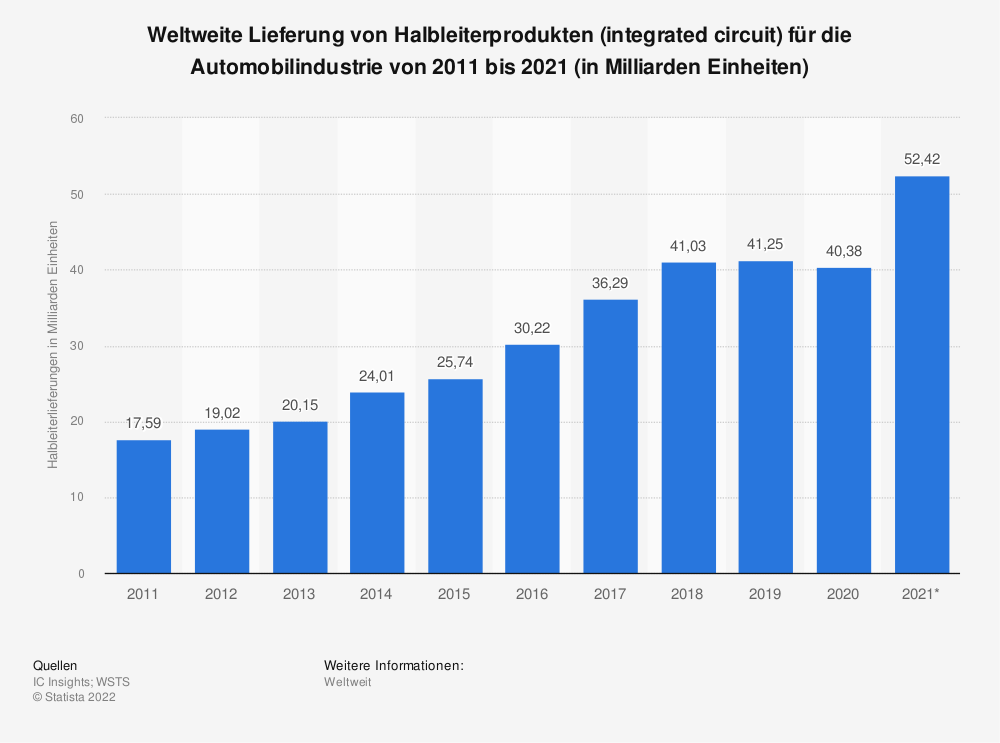
\includegraphics[scale=0.35]{Abbildungen/Martin_Kords_1.png} % 0,9 ursprünglich, auf Seite anpassen
  \caption[M. Kords (2022)] {Weltweite Lieferung von Halbleiterprodukten für die Automobilindustrie von 2011 bis 2021}
\end{figure}
\\
Im Vergleich zur Lage im Jahr 2011 wurden für die Automobilindustrie im Jahr 2021 fast drei mal so viele
Halbleiter geliefert. Ebenfalls mit der Weiterentwicklung von Internet of Things Produkten wird in
Zukunft der Bedarf an Halbleitern weiter steigen.\footcite [Vgl.] []{Bill_McClean} \footcite [Vgl.] []{Voas.2021} \footcite [Vgl.] {Kords.2022}
%Quelle https://www.icinsights.com/news/bulletins/The-Real-Reason-Behind-The-Automotive-Industry-IC-ShortageA-StepFunction-Surge-In-Demand/
\\In diesem Kapitel soll die Preisentwicklung von GPUs betrachtet werden, dabei wird 
ein Zusammenhang geschaffen mit den Ursachen die diese Preisentwicklung 
verursacht haben.
\\

\section{Preisentwicklung}
\label{sec:Preisentwicklung}

Die rapide steigende Preisentwicklung von GPUs ist auf zwei Kernfaktoren reduzierbar.\\
- Größerer Bedarf an GPUs und Halbleitern, dem Kernbestandteil von GPUs\\ %Beispiel aufgezeigt
- Mangelnde Kapazitäten zur Produktion von Halbleitern\\
Der Bedarf an Halbleitern und GPUs ist konstant im Anstieg. Besonders durch die Corona-Pandemie,
hat sich im Vergleich zu 2019 im Jahr 2020 ein Umsatzanstieg von 5,4 \% aufgezeigt.\footcite [Vgl.] []{Voas.2021}
\begin{figure}[h]
  \centering
  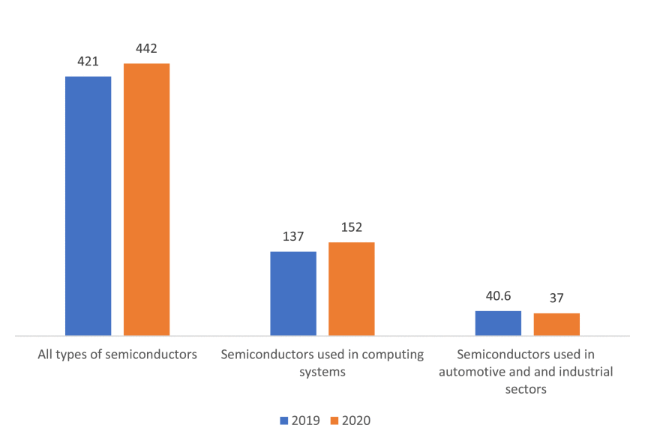
\includegraphics[scale=0.9]{Abbildungen/voas1.png} % 0,9 ursprünglich, auf Seite anpassen
  \caption[Voas, Kshetri und DeFranco (2021)]{Worldwide semiconductor revenues in 2019 and 2020 (dollar, billions)}
\end{figure}
\\Wie in Abbildung 3.2 zu sehen ist, ist der Umsatzanstieg größtenteils durch Erlöse von Computersystemen entstanden.
Im Vergleich dazu sind Umsätze, die durch Abnehmer in der Automobilbranche entstanden sind, gesunken.
Das lässt sich auf den steigenden Bedarf an Computersystemen zurückführen. Während der Pandemie mussten sich
viele Menschen an Home-Schooling und Home-Office anpassen, um weiter den Alltagsbetrieb ausführen zu können.
Ein Nebenläufiger Effekt ist damit, dass durch die Digitalisierung weniger Mobilität benötigt wird.
Damit lässt sich der reduzierte Bedarf an Halbleitern in der Automobilindustrie erklären. Dennoch ist damit insgesamt der Bedarf an 
Halbleitern gestiegen.\footcite [Vgl.] []{Voas.2021}
\\\\ Der steigende Bedarf allein ist aber wie angeführt nicht der einzige Faktor. Die Produktion 
von Halbleitern stagniert. Das lässt sich auf verschiedene Ursachen zurückführen. Da die meisten 
Halbleiter in asiatischen Ländern produziert werden und diese den eigenen Bedarf zuerst decken, ist 
für den Export weniger verfügbar. Ebenfalls haben sich in den letzten Jahren Naturkatastrophen ereignet, die
z.B. durch Dürre, die Produktion lahmgelegten.\footcite [Vgl.] []{Voas.2021}
\\
Durch mangelnde Produktion und steigenden Bedarf hat sich nun ein sehr hoher Marktpreis entwickelt. 
Um diesem entgegenzuwirken ist nicht nur Ressourcenverfügbarkeit zu schaffen, sondern auch eine effizientere Methode zur Nutzung
der Ressourcen.

\section{Ursache Halbleitermangel und Krypto-Mining}
\label{sec:Ursache Halbleitermangel und Krypto-Mining}

Um den Halbleitermangel besser zu verstehen, sollte eine neue Branche, die primär GPU-Leistung 
nutzt, thematisiert werden. Seit dem Jahr 2021 haben Kryptowährungen ein mehr als fünffaches Investitionsvolumen
im Vergleich zum Vorjahr zu verzeichnen.\footcite [] [] {Statista_Research_1}
\\Um den Zusammenhang zu erläutern: Kryptowährungen validieren Ihre Transaktionen durch die Nutzung der 
Blockchain-Technologie. Bei diesem Validierungsprozess werden neue Datenblöcke in einer Datenbank gespeichert und von anderen
Nutzern überprüft durch eine Prüfsumme, die dabei gebildet werden können muss. Um diese Prüfsumme berechnen zu können
nutzen sogenannte "Krypto-Miner" primär GPU-Leistung.\footcite [Vgl.] [S.259-273] {Arslanian.2022}
\\Da große Investitionen für das Kryptomining getätigt werden, hat sich ein neuer Markt mit einer großen Nachfrage gebildet, der
GPUs benötigt.
\\ \\
%Ein Ende in Sicht?
%https://www.gartner.com/en/newsroom/press-releases/2021-05-12-gartner-says-global-chip-shortage-expected-to-persist-until-second-quarter-of-2022
%
Allerdings gibt es faktengestütze Prognosen, welche behaupten, dass der Halbleitermangel nicht zu lange anhalten wird. 
Nach Gartners Prognose für das zweite Quartal 2022 sollte sich der Halbleitermangel verringern, auch wenn dies nicht im vollen Umfang eingetreten ist, sind 
die Argumente für die weitere Zukunft nicht irrelevant.\\
Angeführt wird, dass durch den Halbleitermangel nun die Lieferkette enger überwacht wird.
Daraus resultierend werden mehr Transparenz und Vorinverstionen geschaffen, um die Lieferungen garantieren zu können. 
Ebenfalls möchte man auch die Abnahme von mehreren Lieferanten bevorzugen, anstatt von einem Lieferanten abhängig zu sein.
Diese Faktoren sollen langfristig Sicherheit in der Lieferkette bieten. \footcite [Vgl.] [] {Gartner.2021}

\chapter{Gaming as a Service}
\label{sec: Gaming as a Service}

Gaming-as-a-Service ist ein Zukunftstrend in der Spielindustrie. Je nach Entwicklung, steigt die benötigte Hardwareleistung 
wie CPU, GPU, RAM, sowie Speicherplatz zum Installieren von Spielen stetig an. Hochwertige Spiele können nicht mehr von veralteten 
Computern genossen werden, wodurch die Hardware regelmäßig aktualisiert werden muss, für eine bessere Umgebung. 
\\ \\
In diesem Kapitel soll Cloud Computing mit Gaming-as-a-Service als Beispiel vertieft werden. Hierbei sollen die Funktionalität und Architektur, 
sowie die aktuell verschiedenen Angebote betrachtet werden.


\section{Funktionsweise}
\label{sec:Funktionsweise}

Unabhängig von der Architektur wird das Gaming als Schleifenprozedur betrachtet, die eine Interaktion zwischen Endnutzern und Spiellogik ermöglicht. 
Hierbei stehen zwei wichtige Komponenten in Relation: Der Server, auch Cloud genannt und das Gerät des Endnutzers, auch Thin-Client genannt. Je nach GaaS-Modell, 
findet die Ausführung des Spiels, die Spiellogik und die Wiedergabe der Szenen innerhalb der Cloud statt. Für den Empfang der komprimierten Audio- und Videosignale, 
ist der Thin-Client verantwortlich. \footcite [Vgl.] [] {Zadtootaghaj.2022} In Betracht gezogen werden hier drei GaaS-Modelle: Remote-Rendering-GaaS, Local-Rendering-GaaS 
und Cognitive-Resource-Allocation-GaaS. \footcite [Vgl.] [] {Cai.2014}
\\ \\
Beim Remote-Rendering-GaaS-Modell (RR-GaaS) besitzt die Cloud-Infrastruktur ein Modul zum Kodieren. Dieser ist dafür verantwortlich, jeden Frame der Spielszene zu 
rendern und den Stream des Videos zu komprimieren, damit er an das Thin-Client übertragen werden kann. Dort wird der Stream dekodiert und angezeigt. Benutzereingaben 
werden vom Terminal erfasst und die Cloud an die Spiellogik zurückgesendet, die sich um die entsprechende Aktualisierung des Spielzustands kümmert. \footcite [Vgl.] [] {Dangelo.2015}
Dies impliziert, dass die Hardwareanforderung für den Endnutzern minimiert wird, unabhängig von der Komplexität von Spielszenen, Spiellogik und Interaktionen. Folglich können hochwertige 
Spiele mit leistungsschwachen Geräten bedient werden. \footcite [Vgl.] [] {Cai.2014} Das RR-GaaS-Modell verbraucht jedoch eine beträchtliche Bandbreite, um den komprimierten Videostream 
zu übertragen, und kann besonders empfindlich auf Netzwerkverzögerungen reagieren.
\\ \\
Beim Local-Rendering-GaaS-Modell (LR-GaaS) wird der Stream des Videos in der Cloud als eine Folge von Rendering-Anweisungen auf hoher Ebene kodiert, die zum Thin-Client gestreamt werden. 
Dieser dekodiert und führt die Anweisungen aus, um jeden einzelnen Frame zu zeichnen. \footcite [Vgl.] [] {Dangelo.2015} Der hervorstechendste Vorteil des LR-GaaS-Modells besteht darin, dass 
die Cloud keine einzelnen Frames in Echtzeit mehr über das Internet an die Thin-Clients über-tragen muss, was die Netzwerklast erheblich reduziert. Ansonsten bestehen die ähnlichen Vorteile 
wie beim RR-GaaS-Modell. \footcite [Vgl.] [] {Cai.2014}
\\ \\
Anders als beim RR- und LR-GaaS-Modell, ist beim Cognitive-Resource-Allocation-GaaS die Cloud logisch in eine Reihe von Modulen unterteilt. Die Module können dann wiederum auf dem Thin-Client 
hochgeladen und ausgeführt werden. Das CRA-GaaS-Modell verlagert die Berechnung zurück auf das Client-Terminal und reduziert so die Belastung der Cloud. Die Client-Ressourcen werden effizient 
genutzt, da immer nur die benötigten Komponenten lokal gespeichert werden. Dies ist ein erheblicher Vorteil, wenn man bedenkt, dass die Daten eines kompletten mo-dernen Spiels viel Platz einnehmen.
\footcite [Vgl.] [] {Dangelo.2015}
\\ \\
\begin{figure}[h]
  \centering
  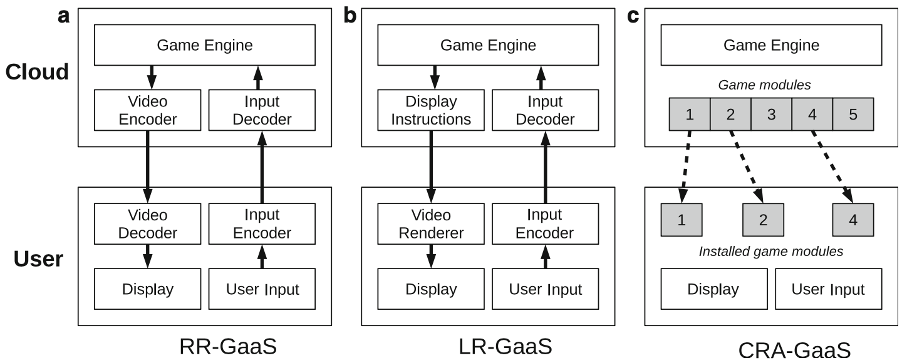
\includegraphics[scale=0.9]{Abbildungen/GaaS_1.png} 
  \caption[D’Angelo, Ferretti and Marzolla (2022)]{Gaming as a Service models}
\end{figure}

\section{Anbietervergleich}
\label{sec:Anbietervergleich}

% Inhalt

\subsection{Voraussetzung}
\label{sec:Vorraussetzung}

All die Prozesse und Interaktionen zwischen der Cloud und dem Thin-Client werden durch die Leistung des Netzwerks eingeschränkt. Weitere Einschränkungen wie eine begrenzte Bandbreite, würde die 
Erfahrung der Spieler beeinflussen. Ist es aber in Deutschland überhaupt anwendbar mit der aktuellen Breitbandverfügbarkeit? Je nach Anbieter und Qualität des Videostreams variiert sich die erforderliche 
Internetgeschwindigkeit. Eines der großen Cloud-Gaming-Anbieter, wie Google Stadia, erfordert eine Bandbreite bei der höchsten Auflösung eine Netzwerkgeschwindigkeit von mindestens 35 Mbit/s. \footcite [Vgl.] [] {Stadia.2022}
Da sich die Cloud beim Gaming-as-a-Service typischerweise im regionalen Netzwerk eines Betreibers befinden, bleibt die Ende-zu-Ende-Übertragungsverzögerung gering, da zwischen dem Client und dem Server normalerweise viel Bandbreite verfügbar ist. 
Falls jedoch mehrere Geräte den Breitbandanschluss zu Hause nutzen, kann die verfügbare Bandbreite beim Zugang auf der letzten Meile erheblich variieren.
\\ \\
\begin{figure}[h]
  \centering
  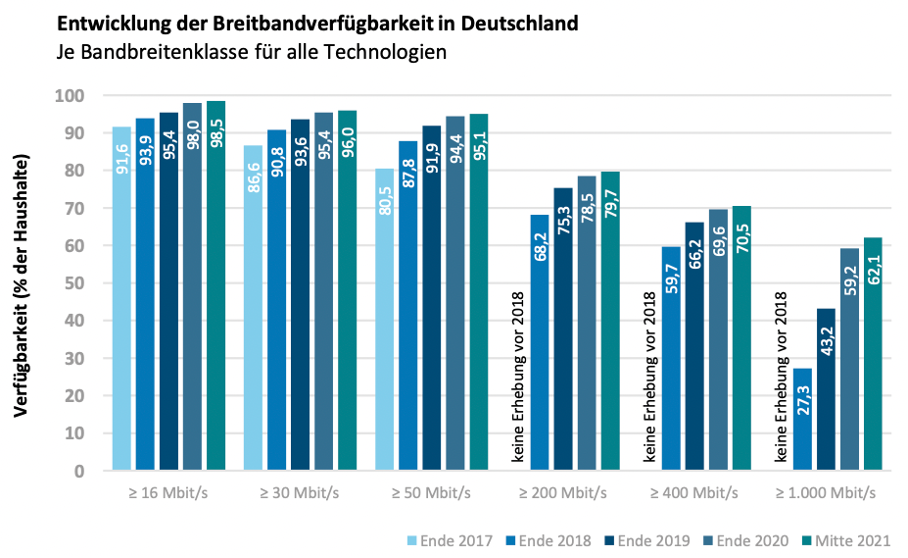
\includegraphics[scale=0.9]{Abbildungen/GaaS_2.png} 
  \caption[atene KOM GmbH (2021)]{Entwicklung der Breitbandverfuegbarkeit in Deutschland nach Bandbreitenklassen}
\end{figure}
\\ \\
Aus der Abbildung 4.2: „Entwicklung der Breitbandverfügbarkeit in Deutschland“ ist ein Zuwachs der Breitbandverfügbarkeit in den vergangenen Jahren deutlich zu sehen. Ein deutlicher Sprung ist in der 
höchsten Klasse zu sehen, die sich mehr als verdoppelt hat. Festzustellen ist also, dass die entnommene Anforderung von Google Stadia mit 35 Mbit/s für die höchste Auflösung 
von 95,1 Prozent der Haushalte in Deutschland erfüllen.

\subsection{Angebot}
\label{sec:Angebot}

Aktuell sind fünf große Cloud-Gaming-Anbieter im deutschen Markt vertreten: Nvidia GeForce Now, Google Stadia, Shadow, Xbox Cloud-Gaming, PS Now sowie weitere kleine Anbieter.  Für die Nutzung des Angebotes 
der Anbieter ist ein Abonnement erforderlich und nur mit bestimmten Geräten nutzbar. Erste Unterschiede ergeben sich bei den jeweiligen Konzepten. Vergleicht man die angebotenen Abos des Anbieters Nvidia GeForce 
Now mit Google Stadia, bietet Nvidia GeForce Now drei mögliche Mitgliedschaften, bei der man je nach Auswahl unterschiedliche Leistungen erhält. \footcite [Vgl.] [] {Suznjevic.2016}
Im Vergleich bietet Google Stadia nur einen möglichen Abo, bei der jeder Endnutzer die gleichen Kosten und Leistungen angeboten bekommt. Aufgrund der Diversität im Angebot besteht im Konzept der einzelnen Betreiber 
immer noch eine Gemeinsamkeit. Und zwar schaffen die Konzepte einen potenziellen Markt für Benutzer, die nicht den Kauf von Spielsoftware, sondern den Kauf von Spielzeit für Computer- und Konsolenspiele anzustreben.
Auf diese Weise können Benutzer zu geringen Kosten auf eine Vielzahl von Spielen zugreifen.
\\ \\
Von den großen Cloud-Gaming-Anbietern ist kein deutsches Unternehmen mitinbegriffen, zumindest aktuell nicht mehr. Auch Telekom hatte eine eigene Cloud-Gaming-Plattform, bei der keine Downloads oder Kauf teurer 
Hardware von Nöten ist. Nach nicht einmal zwei Jahren, wurde der Streamingdienst eingestellt, aufgrund Desinteresses der Spieler. \footcite [Vgl.] [] {Telekom.2022} Laut Prognose wird der Marktwert von Cloud-Gaming 
weltweit bis 2024 sich um 4,27 Prozent steigern. \footcite [Vgl.] [] {Clement.2022} 

\subsection{Preis}
\label{sec:Preis}

Die Preisgestaltung variiert sich von Anbieter zu Anbieter, von Kostenlos bis zu 29,99 Euro pro Monat. Hier spielen zwei große Faktoren eine Rolle: Service/Leistung und Spielebibliothek. Bei der Mitgliedschaft 
„Kostenlos“ ist eindeutig festzustellen, dass diese Option nur für Interessenten ist, die zum Testen des Service angeregt werden. Mit einem Abo von 9,99 Euro im Monat, wird natürlich schon bei einigen Anbietern der volle Umfang geliefert.

\section{Hardwarevorraussetzung um Usability zu gewährleisten}
\label{sec:Hardwarevorraussetzung um Usability zu gewährleisten}

Die Anforderungen an Rechenleistung und Speicherkapazität von Computer- und Videospielen werden immer höher, da die Spiele immer realistischer und komplexer werden. \footcite [Vgl.] [] {Laulajainen.2006} Für einen einfachen Heimcomputer ist das 
Abspielen von hochwertigen Spielen in einer guten Umgebung nicht mehr möglich und muss aktualisiert werden. \footcite [Vgl.] [] {Suznjevic.2016} Für die Nutzung des Cloud-Gaming reicht das jedoch. Je nach Anbieter sind die Systemanforderungen 
unterschiedlich, aber dennoch keine hohen Anforderungen. 
\\ \\
Nehmen wir als Beispiel eines der größten Cloud-Gaming-Anbietern Nvidia GeForce Now (GFN). Um GFN nutzen zu können, werden GPUs, die seit 2015 veröffentlich wurden, beim Streaming mit 
bis zu 3840x2160p 60 FPS und 1440p/1600p 120 FPS unterstützt. Für die CPU genügt eine Dual-Core x86-64 mit 2,0 GHz und RAM mit nur 4 GB Speicher. Mit der Mindestanforderung von GFN muss der Thin-Client keine große Verarbeitungsleistung und 
Speicherkapazität haben. \footcite [Vgl.] [] {Clement.2022} 
Mit nur niedriger Anforderung kann alte Hardware die Usability bei Spielen wie bei High-End-Computern gewährleistet werden. Es besteht keine Sorge um die Prozessorleistung, das Betriebssystem, die Grafikkarten oder andere technische 
Spezifikationen eines Computers. \footcite [Vgl.] [] {Ojala.2011}

\chapter{GPU as a Service}
\label{sec:GPU as a Service}

Außerhalb von Gaming as a Service gibt es weitere Service-Möglichkeiten die ebenfalls GPU as a 
Service beanspruchen bzw. inkludieren. Wachsende Märkte dafür sind
das Rendern von 3D-Modellen und animierten Videos, 
wie auch Deep-Learning-Model-Training für KIs. 
\\Im folgenden Kapitel wird erläutert werden, wie GPU as a Service-Anbieter Ihren Service 
realisieren können und Qualität mit verschiedenen Methoden schaffen. Wie auch Einsatzgebiete 
für Cloud-Lösungen festgestellt und identifiziert werden.

\section{Funktionsweise}
\label{sec: Funktionsweise}

Bei der Dienstleistungsinanspruchnahme werden die von einem Nutzer geforderten
Prozesse, wie z.B. das Rendern von 3D-Modellen, durch die Rechenleistung des 
Anbieters verarbeitet. Im Gegensatz zu der Privatnutzung bei der nur eine GPU genutzt wird, 
verwenden GPU a as Service-Anbieter mehrere GPUs. 
Allerdings, da GPUs nur als Co-Prozessoren in solchen Systemen genutzt werden, 
können diese nicht eigenständig betrieben werden, sondern benötigen ein zentrales 
Betriebssystem, welches auch als Kernel bezeichnet. Üblicherweise wird dies skalierbar angewendet mit einer
Vielzahl an Kernels, welche eine Vielzahl an GPUs besitzen.\footcite [Vgl.] [] {Wang.2017}
\\% auskommentiert für Textmessen
\begin{figure}[h]
 \centering
  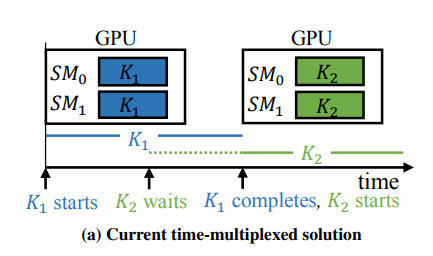
\includegraphics[scale=1.4]{Abbildungen/wang1.png} 
  \caption[Wang u. a. (2017)]{Current time-multiplexed solution}
\end{figure}
\\%
Es gibt verschiedene Methoden, diese Prozesse zu verarbeiten. Eine Methode davon 
ist das Zeit-Multiplexverfahren. Bei diesem Verfahren werden mehrere Prozesse auf die Kernels
sequenziell aufgeteilt und verarbeitet, wie in Abbildung 5.1 zu sehen. Dieses Methode 
hat keinen direkten Mehrwert in Bezug zur Verarbeitungseffizienz, allerdings verhindert 
sie, dass Prozesse Kernels unnötig blockieren können. \footcite [Vgl.] [] {Wang.2017}
\\ \\
%Andere Methode erklären aus der selben Quelle
Ein anderer Ansatz, um Konstanz zu schaffen, ist, dass man die Kernels über Software zu einem Kernel fusioniert. 
Das ist vergleichbar mit dem für Festplatten verwendeten "redundant array of independent disk"-System, auch abgekürzt RAID genannt, 
welches gängiger bekannt ist. Durch das Fusionieren der Kernels über die Software kann eine 
konstante Leistung gewährleistet werden.
Ebenfalls, um eine Fairness zwischen allen Leistungsabnehmern zu schaffen, 
da es keine Situation geben kann, einen leistungsschwächeren Kernel zugewiesen zu bekommen.\footcite [Vgl.] [] {Wang.2017}
\\ \\
Eine quasi gegenteilige Methode, die Kernels in verschiedene Partitionen aufzuteilen, anstatt Sie zu fusionieren.
Wieder mal vergleichbar, wie man auch mit Festplatten umgehen kann. Die Leistung des Kernel wird 
in verschiedene Partitionen aufgeteilt. Diese können dann je nach Monetarisierungsmodell 
vermietet werden, für einen Zeitraum oder auf einer Bedarfsbasis. Daraus entsteht der Vorteil, 
dass Nutzer des Services ihren Bedarf selbst definieren können und garantiert diese Leistung 
in Anspruch nehmen können. \footcite [Vgl.] [] {Wang.2017}
\\ \\
Es gibt neben diesen Methoden weitere Maßnahmen für die Qualitätssicherung des GPU as a Service Modells. 
Allerdings würden diese sich zu weit vertiefen und über das Ziel dieser Arbeit hinausgehen. 
Für eine weitere Vertiefung ist die Arbeit von Wang u.a., “Quality of Service Support for Fine-Grained Sharing on GPUs”. zu empfehlen.

\section{Einsatzgebiete}
\label{sec: Einsatzgebiete}

%Wachsende Märkte dafür sind
%das rendern von 3D-Modellen und animierten Videos, 
%wie auch deep learning model training für KIs.

Die Einsatzgebiete sind weitreichend und können auf zwei Bedarfsmethoden eingeteilt werden.
Einmal in Schüben, in denen ein festes Ziel und der Aufwand definiert werden, welche der Prozess erreichen soll.
Beispiele dafür sind Rendern von 3D-Modellen und animierten Videos.
\\ 
Um dieses Beispiel auszuführen: Wenn ein 3D-Modell dargestellt wird, besteht es aus Matrixoperationen, die von GPUs 
in der Regel berechnet werden. Dies hat meist das Ziel, diese realitätsgetreu und logisch in einer Umgebung darzustellen.
Dieses Beispiel lässt sich auf animierte Videos erweitern, bei denen dann eine veränderte Version des Vorgängermodells oder ein 
vollkommen anderes Modell für jedes Bild im Video dargestellt wird. \footcite [Vgl.] [] {Loop.2006}
\\ \\
Ebenso ist es möglich, dass mit einem optionalen Ziel, aber unbekannten Aufwand, so ein Prozess ausgeführt wird. 
In diesem Fall wird eine konstante Rechenleistung benötigt.
Beispiele dafür sind Deep-Learning-Modelle für KIs oder Gaming as a Service.
\\
Um auch hier ein Beispiel anzuführen, falls Gaming as a Service-Dienste in Anspruch genommen wird.
Bei diesem Service ist kein Ziel festgelegt, da auch kein konkreter Prozess vorgegeben ist.
Anhand der Eingaben des Nutzers variiert die benötige Visualsierung und Spielelogik. Da die Eingaben 
nicht vorher konkret bekannt sind, besteht ein konstanter Bedarf an Rechenleistung um auf die Eingaben 
reagieren zu können. Die Rechenleistung wird benötigt bis der Nutzer das Spiel beendet. \footcite [Vgl.] [] {Lattuada.2022} \footcite [Vgl.] [] {Wang.2017} \footcite [Vgl.] [] {Loop.2006}
%Schlussfolgerung aus eigenem Wissen und den Papers

\section{Vergleich eigene GPU und GPU in der Cloud}
\label{sec:Vergleich eigene GPU und GPU in der Cloud}

Nach den angeführten Informationen lässt sich Folgendes feststellen:  
Der Bedarf an GPU Rechenleistung ist im konstanten Wachstum für verschiedene Märkte. Die GPU as a Service-Anbieter 
können Ihre Systeme entsprechend dem Monetarisierungsmodell und den Leistungsprioritäten aufstellen. 
Dabei handelt es sich nicht um neue Methoden, sondern um etwas mit der Massenspeicherverwaltung Vergleichbaren. 
Je nach geplanter Nutzung werden GPUs entweder in Schüben oder mit konstanter Rechenleistung beansprucht.\\ \\
Nach unserem Ermessen spielt besonders bei der Entscheidung zwischen der eigenen GPU und GPU as a Service die 
benötigte Rechenleistung und die Verfügbarkeit des Services eine Rolle. Unter der Annahme, dass der Dienstleister des GPU as a Service permanent 
verfügbar ist. Für Prozesse, welche in Schüben erfolgen und große Rechenleistung benötigen, ist GPU as a Service ein attraktives Angebot.
Diese können dadurch in kurzer Zeit abgeschlossen werden.\\ \\
Eine eigene GPU ist attraktiver im Fall von konstant benötigter Rechenleistung, wenn eine verfügbare GPU in der Lage ist, 
die benötigte Rechenleistung zu erbringen. Andernfalls ist GPU as a Service ebenfalls eine Lösung, besonders in Zeiten,
in denen die Preise von GPUs mit dem Halbleitermangel gestiegen sind.

\chapter{Marktvorhersage}
\label{sec:Marktvorhersage}

%Inhalt
Die Gaming-Industrie ist in den letzten Jahren stetig gewachsen und wird auch in Zukunft weiter
wachsen. In Abbildung 6.1 werden die Umsätze der Gaming Industrie mit einer Prognose für das Jahr 2024 dargestellt.
Nach Newzoo betrug der Umsatz der gesamten Gaming-Industrie im Jahr 2021 192,7 Milliarden
US-Dollar und wird bis 2024 auf 222,6 Milliarden US-Dollar ansteigen. Von 2020 bis 2024 wird 
von einem durchschnittlichem, jährlichem Wachstum in Höhe von 5,6 Prozent ausgegangen.
\\% auskommentiert für Textmessen
\begin{figure}[h]
 \centering
  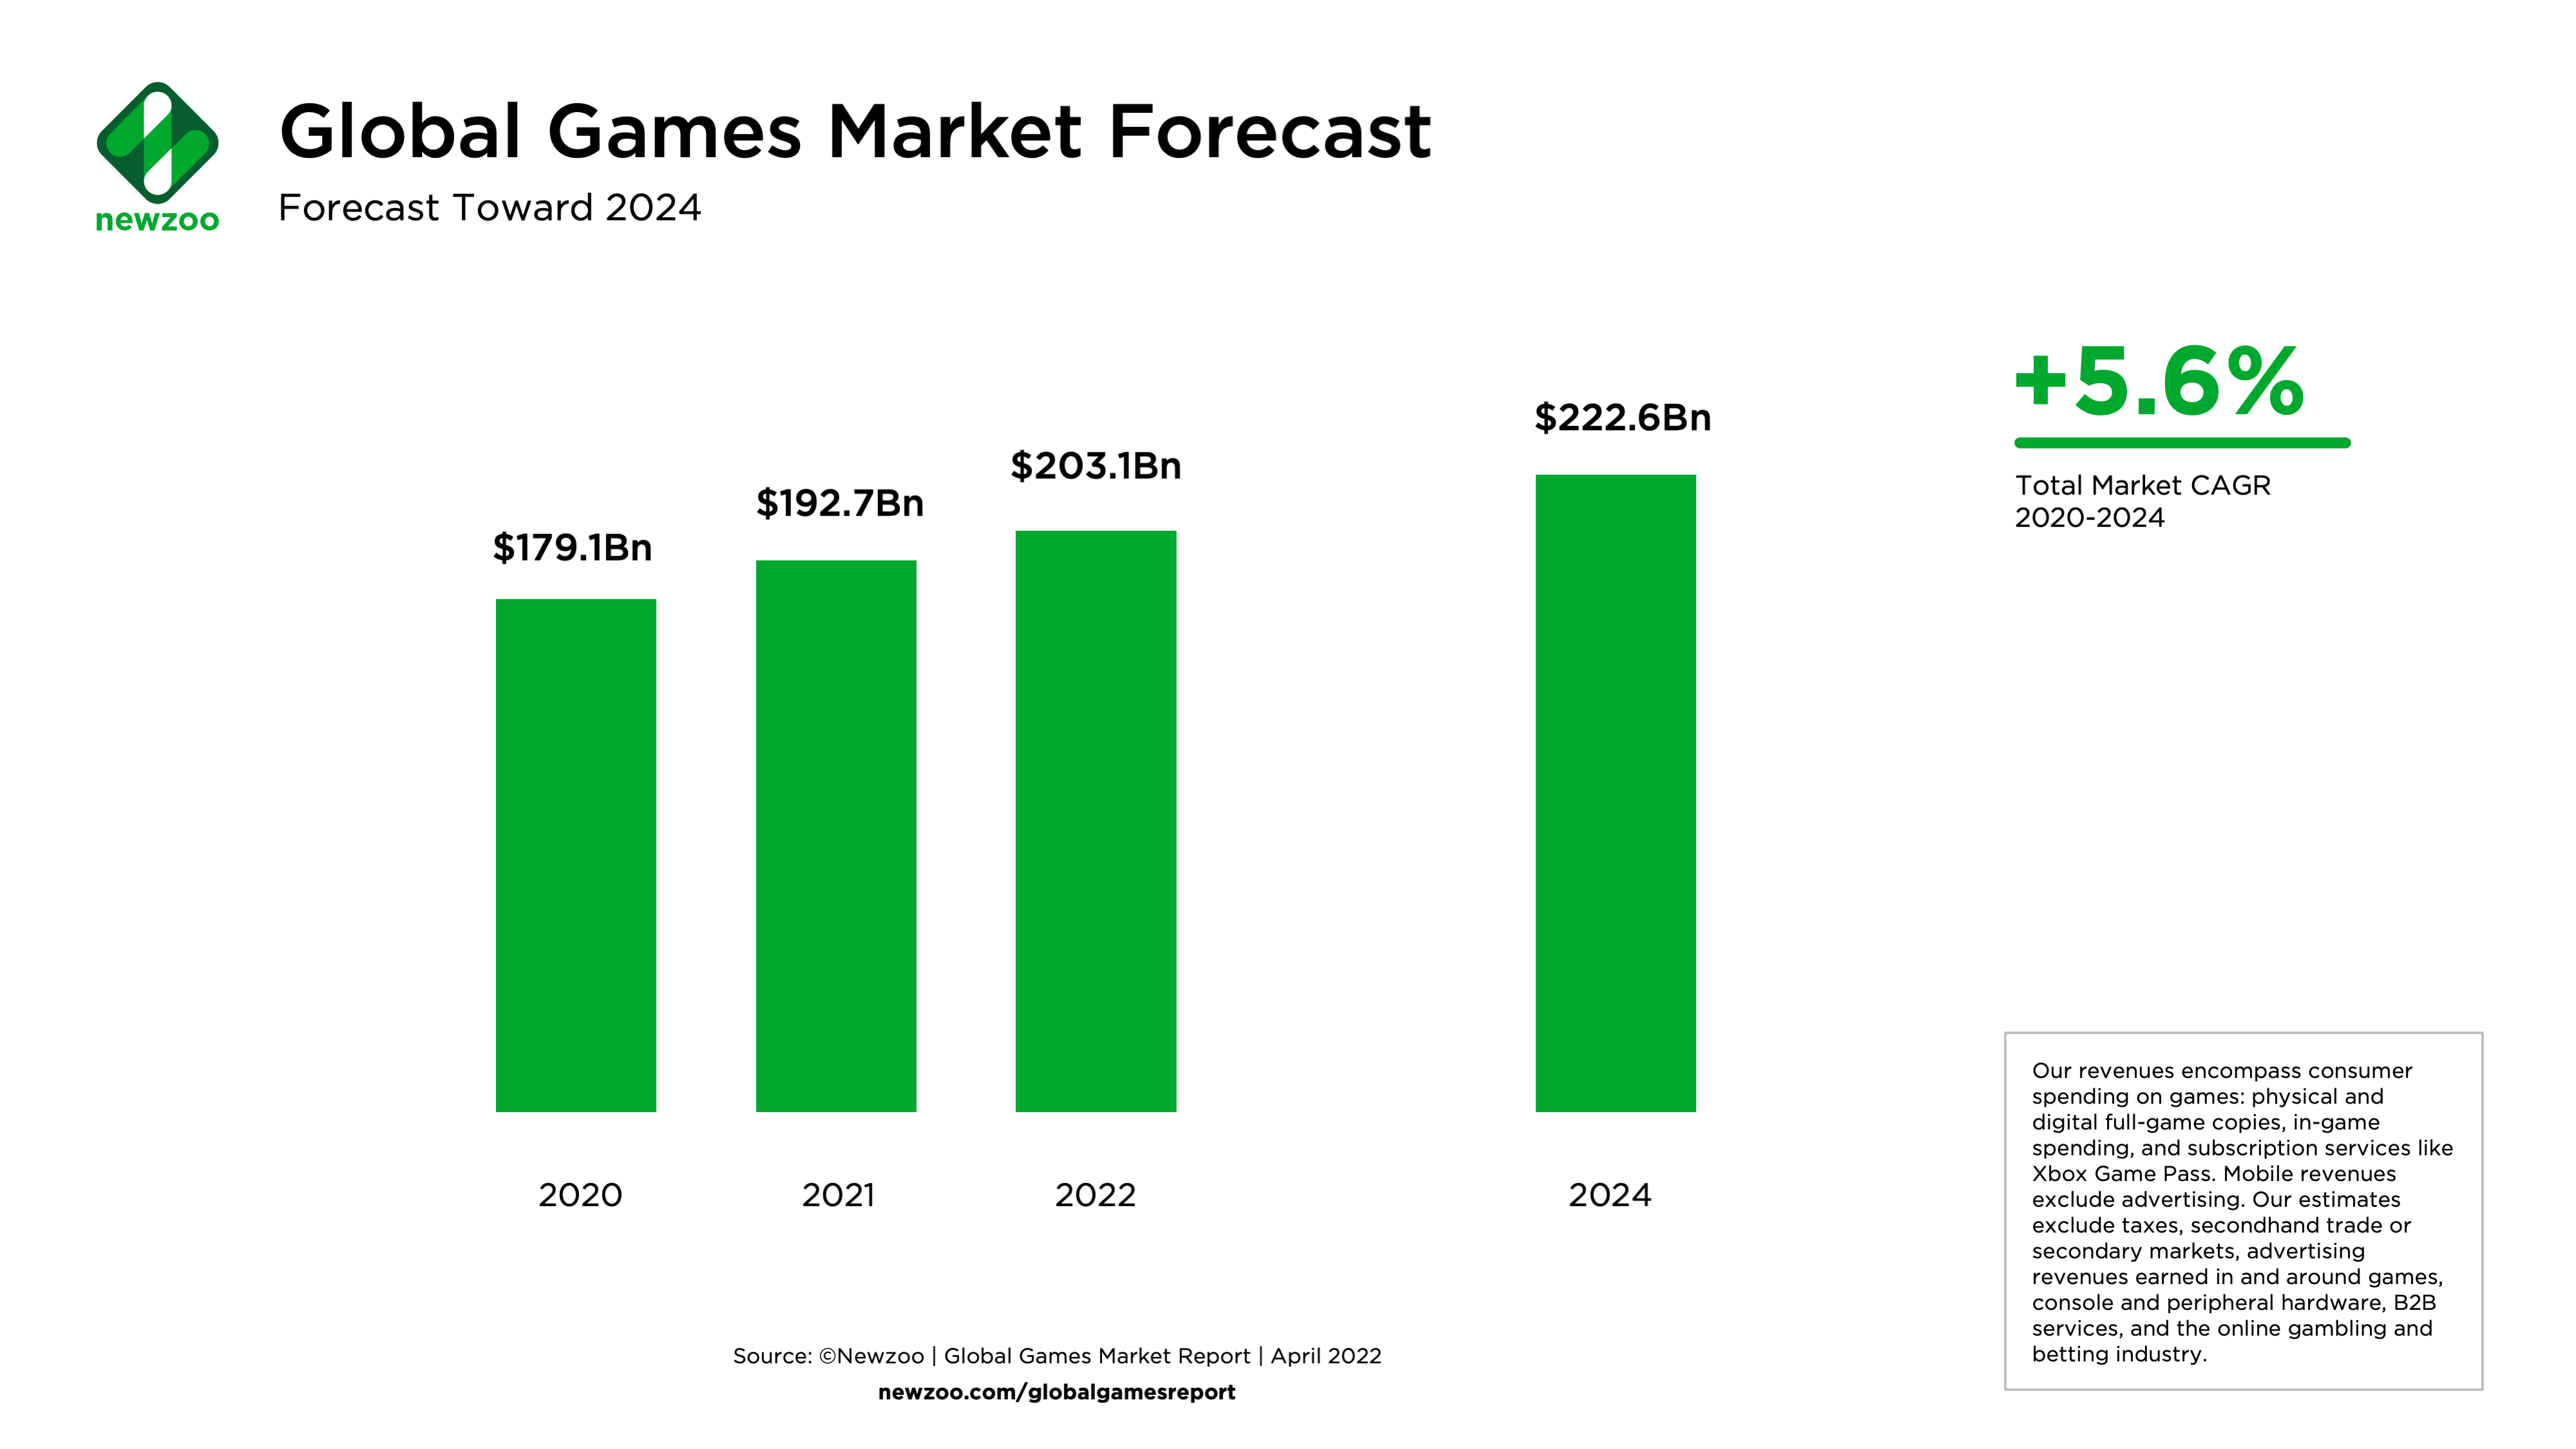
\includegraphics[scale=0.12]{Abbildungen/Newzoo_Global_Games_Revenue_Forecast-2.png} 
  \caption[Newzoo]{Umsatz mit Cloud Gaming 2019-2021 und Prognose für 2024}
\end{figure}
\\%

Auch bei den jährlichen Spielerzahlen, geht Newzoo von einer Steigerung aus. Mit einer jährlichen 
Wachstumsrate von 5.6 Prozent steigen die Spielerzahlen von 2,33 Milliarden Spielern, im Jahr 2015,
zu einer Prognose von 3,32 Milliarden Spielern, für das Jahr 2024. Bemerkenswert an dieser Statistik
ist die Aufschlüsselung der Spieler nach Endgeräten in 2022. Demnach ist ein Großteil der Spieler, 
2,9 Milliarden, auf dem Handy aktiv. Die zweitmeisten Spieler, 1,4 Milliarden, nutzen einen PC, Während
auf Konsolen, mit 900 Millionen aktiven Spielern, vergleichsweise wenige Spieler aktiv sind. 
Die Summe dieser Zahlen stimmt nicht mit der Gesamtzahl an Spieler in 2022 überein, da ein Spieler 
auf mehreren Endgeräten aktiv sein kann. 

Im Jahr 2022 waren 94 Prozent aller Spieler auch auf dem Handy aktiv. Für das Cloud Gaming ist dies interessant,
weil, durch die Verlagerung der Rechenpower vom Endgerät in die Cloud, immer mehr Spiele auf dem Handy spielbar werden, für
die in der Vergangeheit ein leistungsstarker PC oder eine Konsole benötigt wurden. So kann sich in Zukunft für Handyspieler 
einer größere Auswahl an Spielen eröffnen. Gleichzeitig bekommen Publisher und GaaS-Provider Zugang zu einer neuen potentiellen
Zielgruppe.
\\% auskommentiert für Textmessen
\begin{figure}[h]
 \centering
  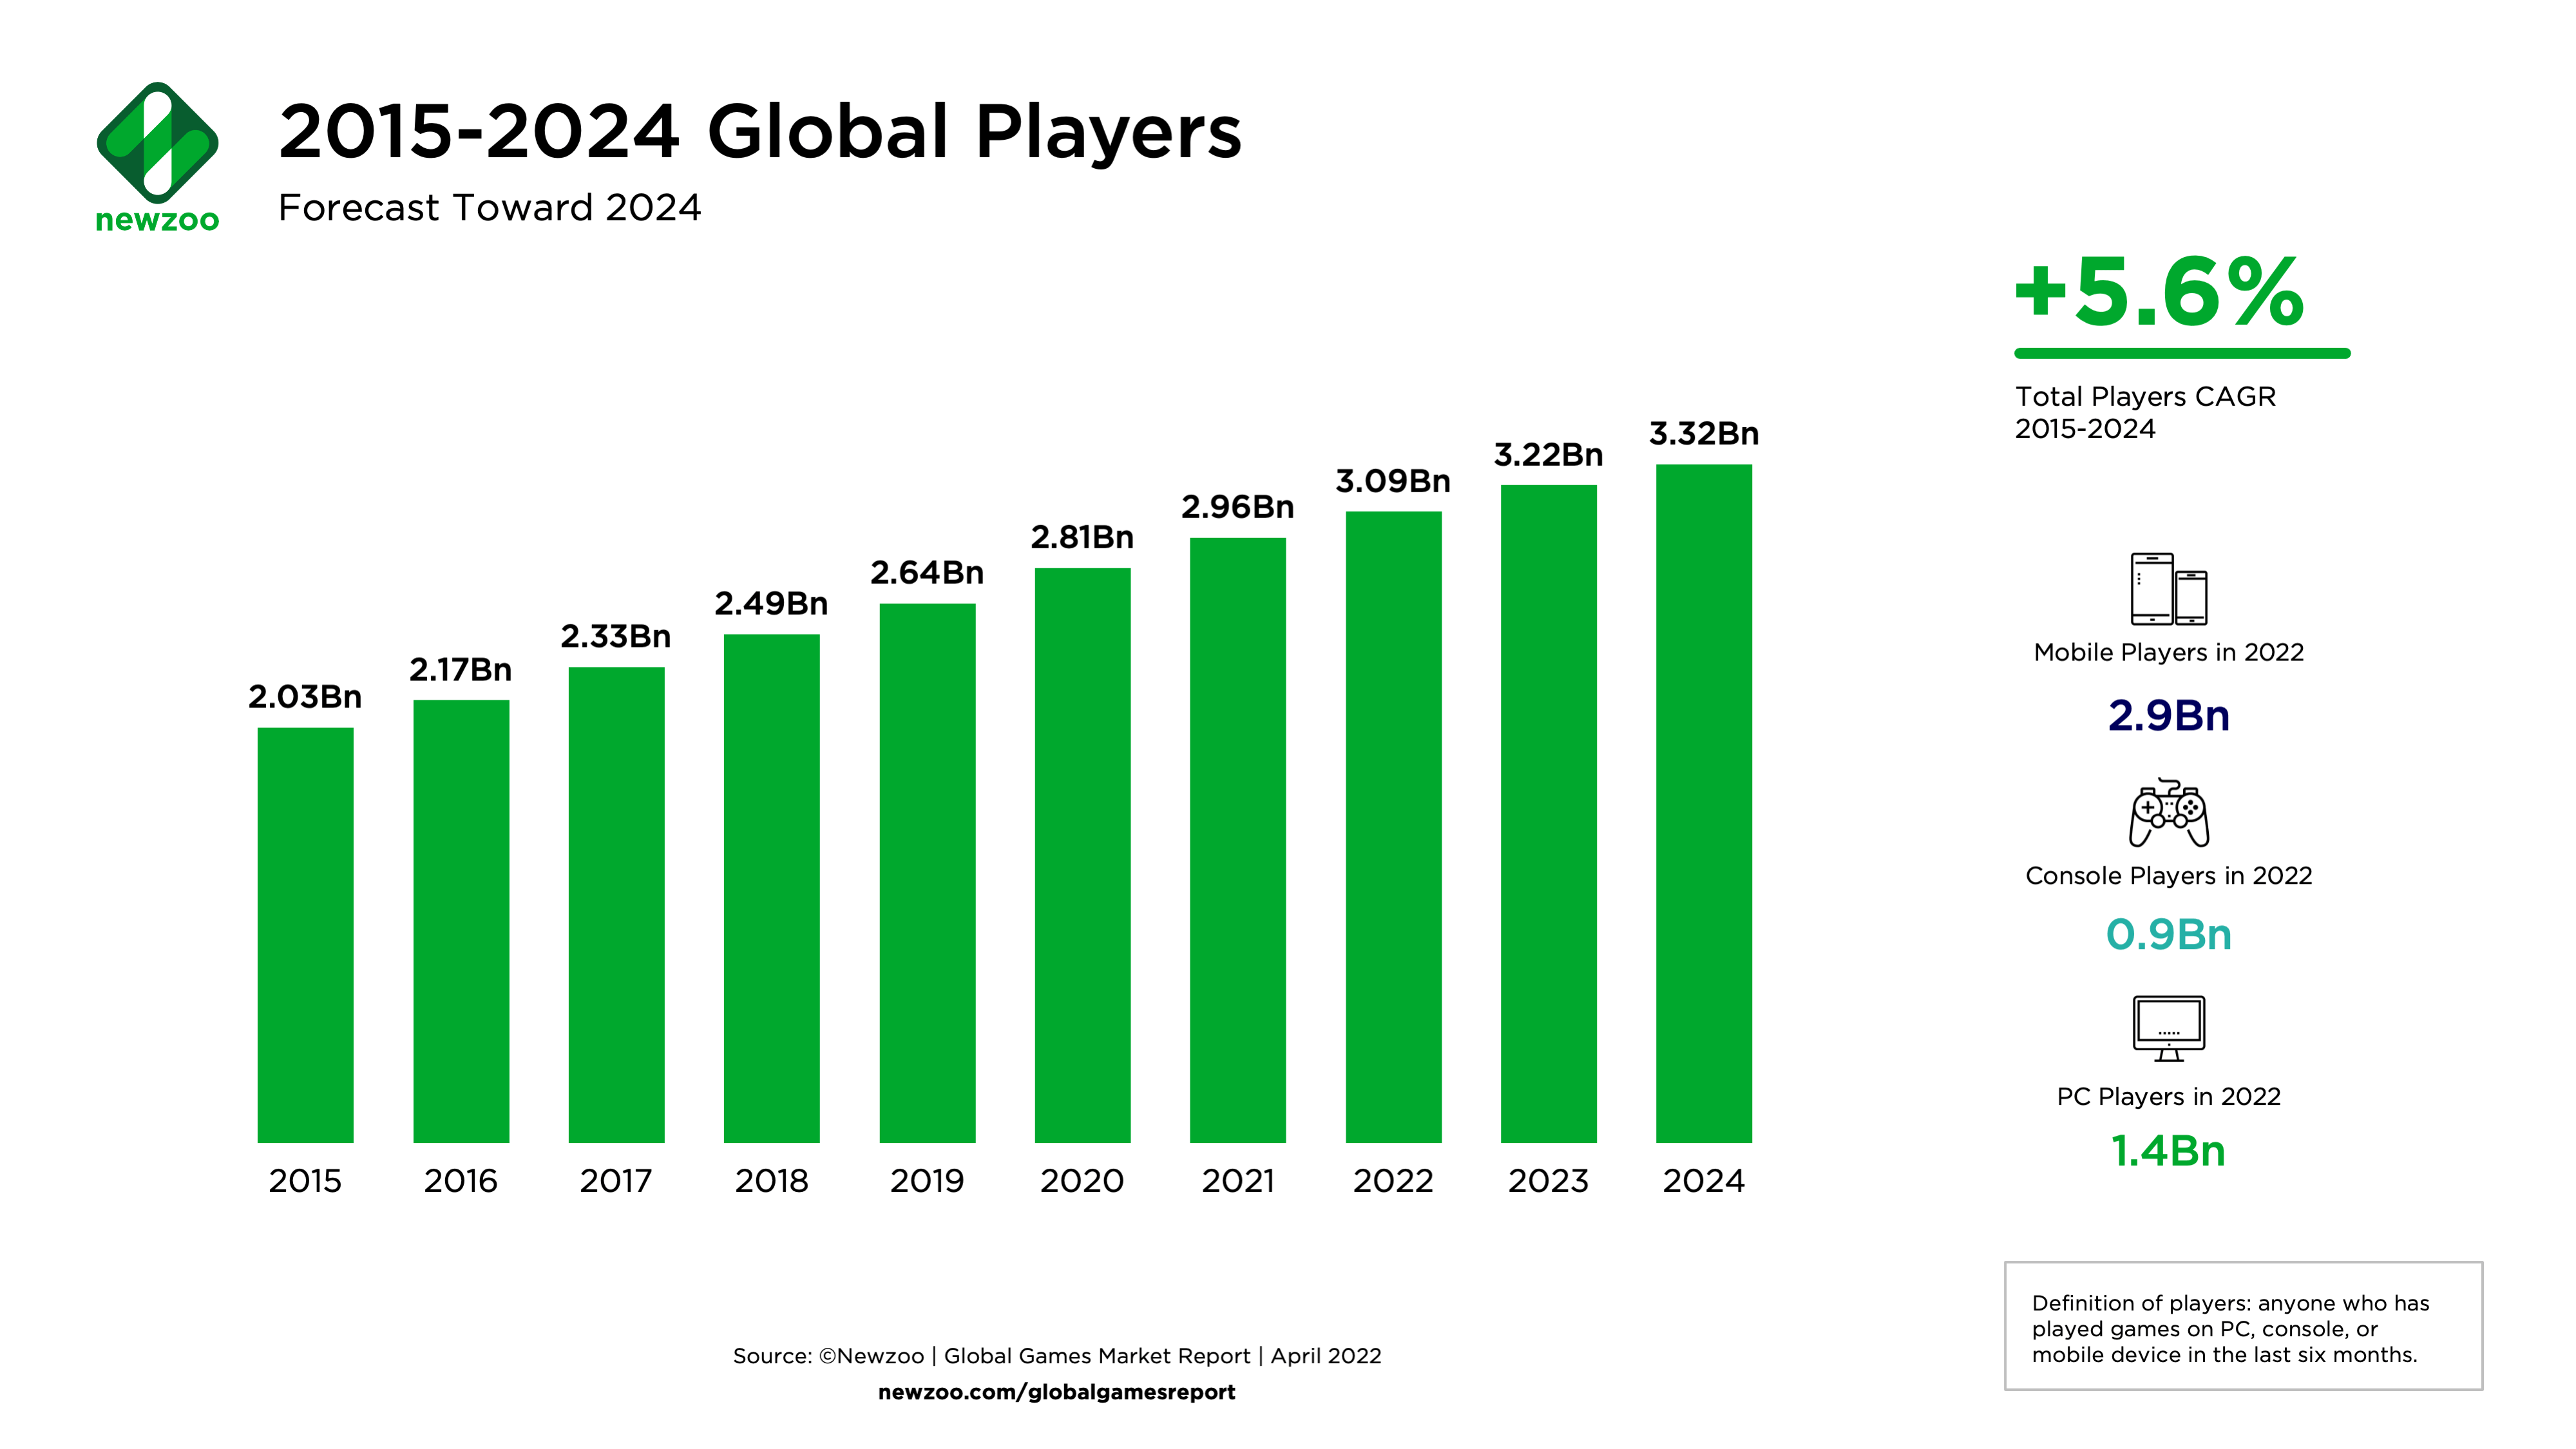
\includegraphics[scale=0.12]{Abbildungen/Newzoo_Global_Players_Forecast.png} 
  \caption[Newzoo]{Prognose Spielerzahlen bis 2024}
\end{figure}
\\%

Im Bereich Cloud Gaming, bzw. Gaming as a Service, wird in den kommenden Jahren ein signifikanter/bemerkenswerter
 Anstieg erwartet. Im Jahr 2021 nutzten etwa 21.7 Millionen Menschen Angebote im Bereich Cloud Gaming, dadurch konnte ein
 Umsatz in Höhe von etwa 1,5 Milliarden US-Dollar erwirtschaftet werden (Newzoo Article). Die Prognose von Newzoo für das Jahr 
 2024 geht von einer Verdreifachung der Nutzerzahlen aus, während sich die Umsätze vervierfachen sollen. Damit würden knapp 60
 Millionen Spieler Cloud Gaming Angebote nutzen und einen Umsatz in Höhe von 6,3 Milliarden US-Dollar generieren(Newzoo). Als Hauptgrund für den erwarteten Wachstum wird angeführt, dass sich die Technologie als rentabel und brauchbar bewiesen hat. Dadurch wurde der Weg geebnet, sodass 
 der Markt in Zukunft schneller wachsen kann.
\\% auskommentiert für Textmessen
\begin{figure}[h]
 \centering
  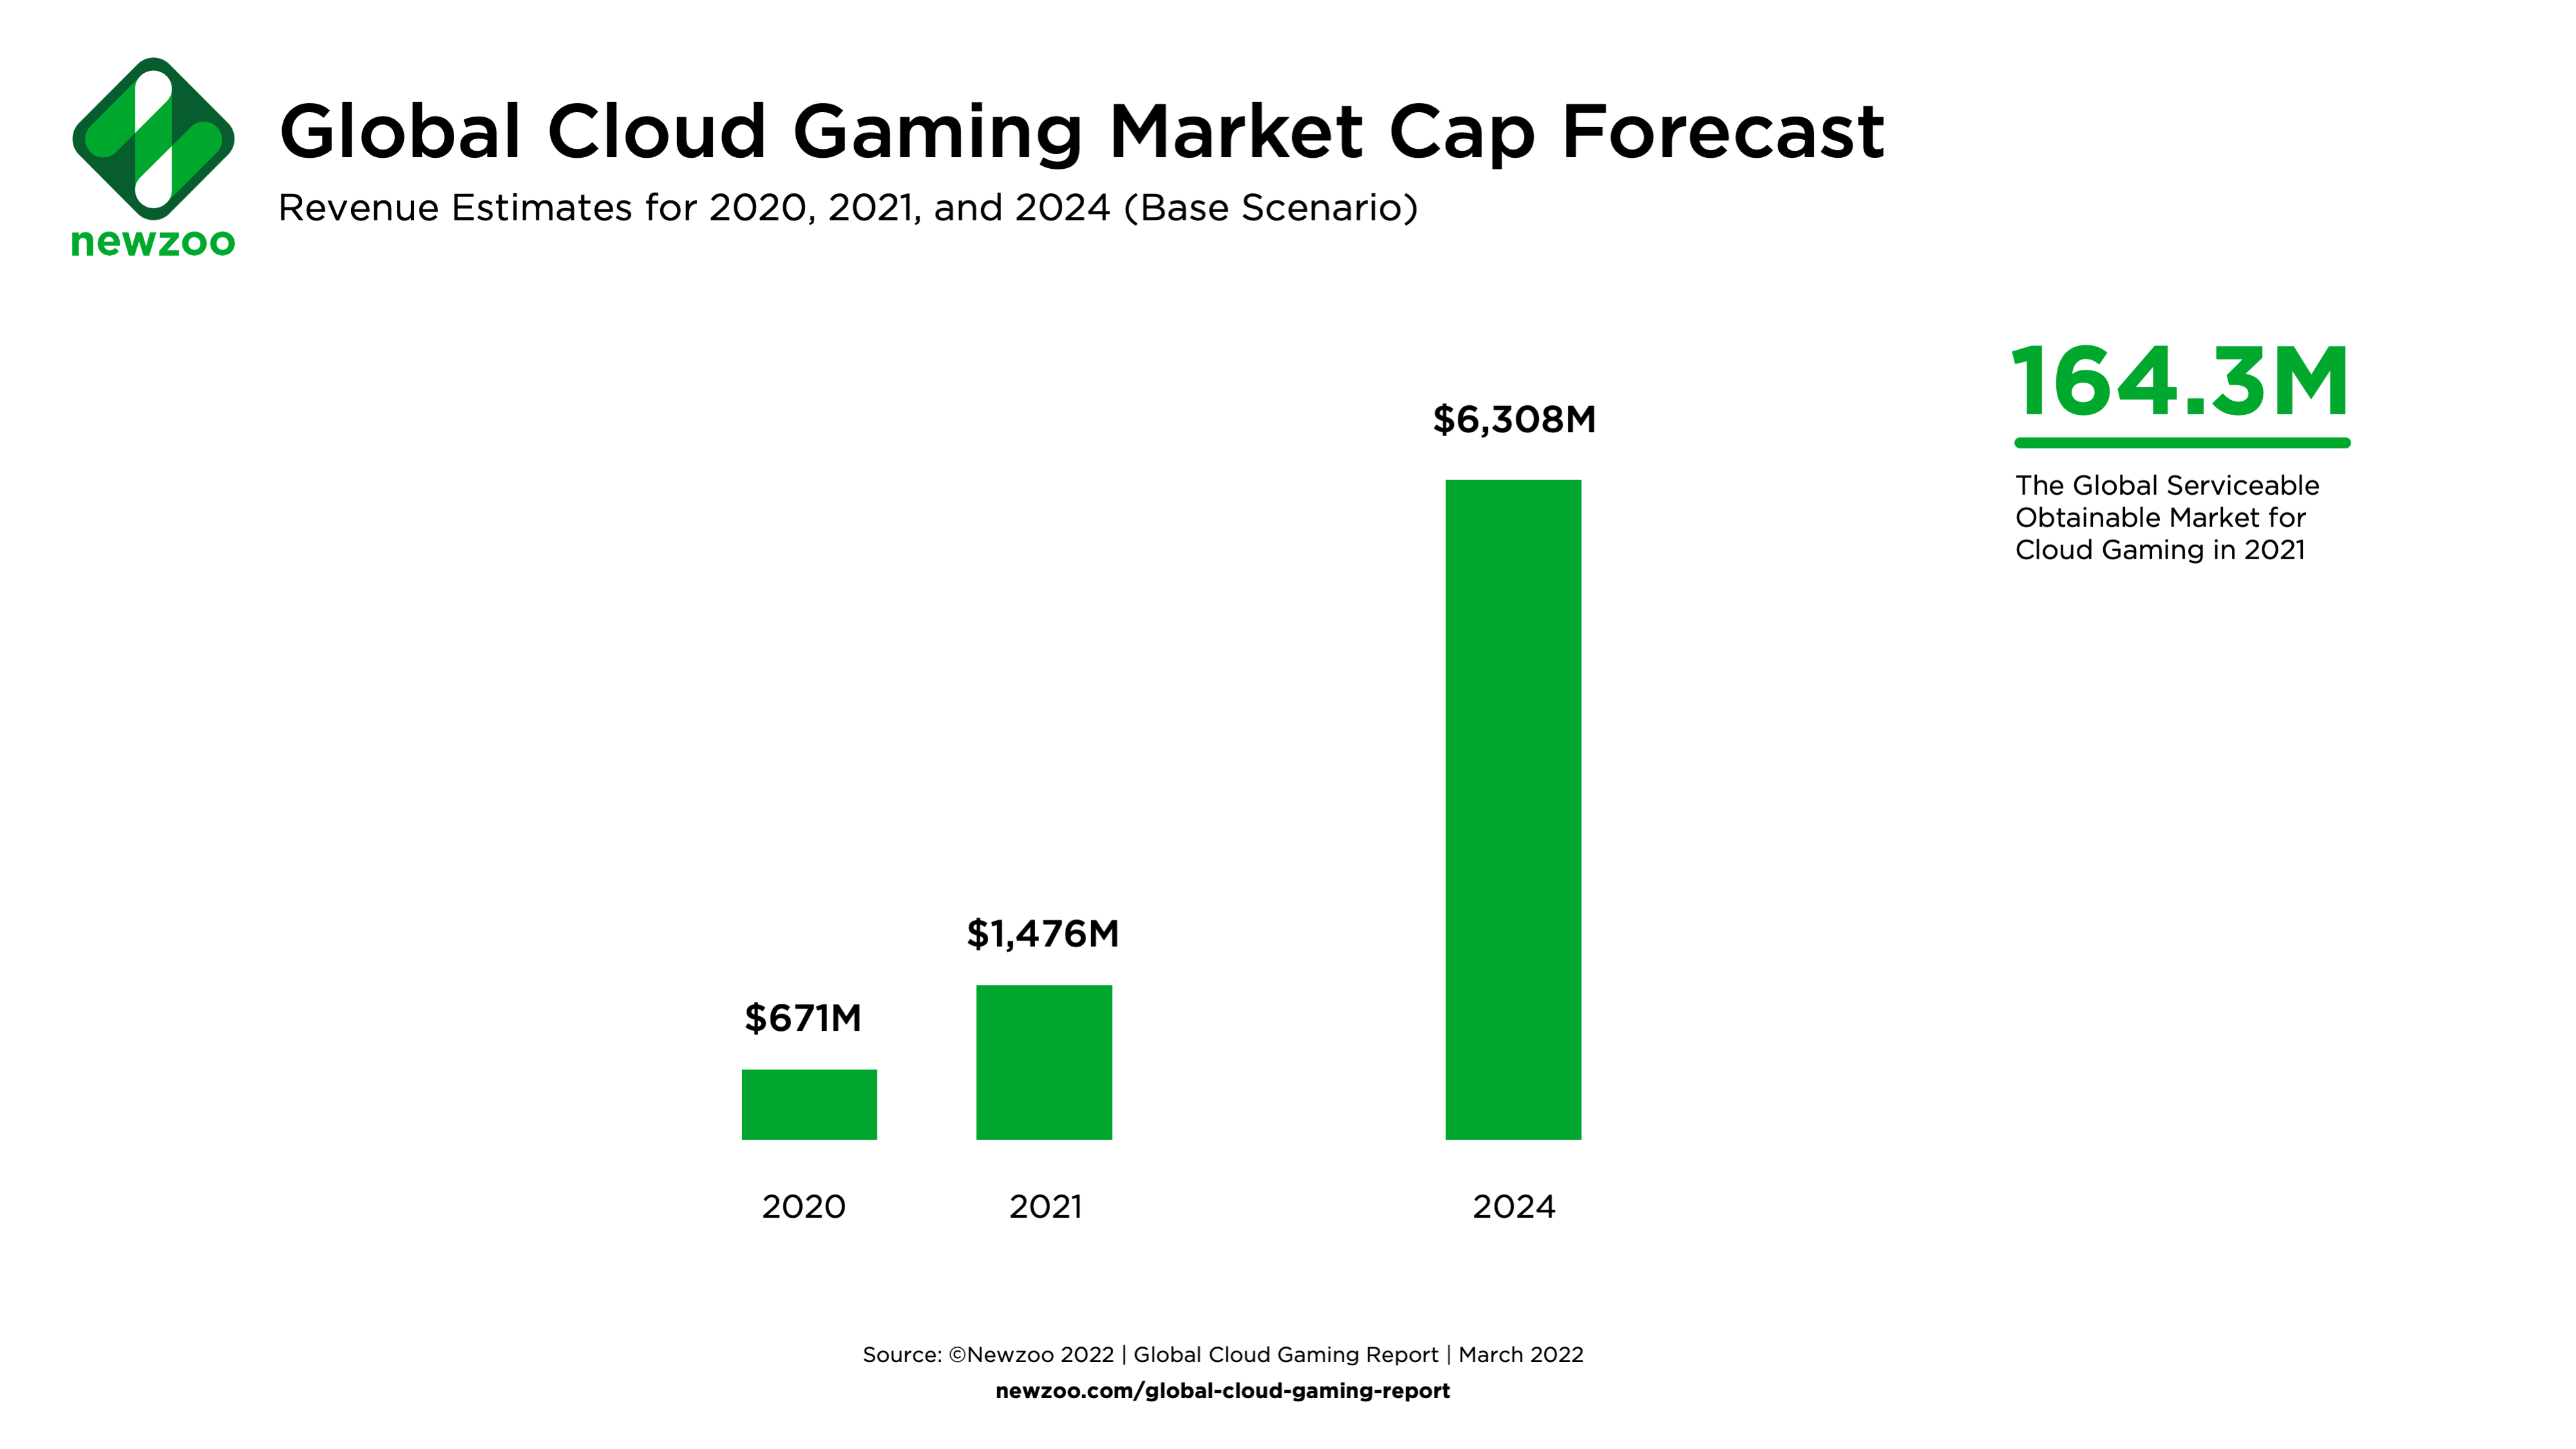
\includegraphics[scale=0.12]{Abbildungen/Newzoo_Global_Cloud_Gaming_Market_Cap_Forecast_March2022.png} 
  \caption[Newzoo]{Umsatz mit Cloud-Gaming 2019-2021; Prognose für 2024}
\end{figure}
\\%

Es gibt viele aktuelle Cloud-Gaming Trends, die zu diesen optimistischen Prognosen führen. So konnten Cloud Gaming Provider 
Partnerschaften mit Kommunikation und Internetanbietern in Südostasien, sowie Lateinamerika abschließen. Dadurch soll in diesen, 
ohnehin bereits wachsenden, Gaming Märkten Cloud Gaming gestärkt werden (Newzoo). 

Aber auch die anhaltend hohen Preise im Grafikkartenmarkt
spielen eine Rolle. Endnutzer können, oder wollen, sich die hohen Preise auf dem Resellermarkt oft nicht leisten, während es nahezu 
unmöglich ist eine Grafikkarte zum Listenpreis erwerben zu können. Unternehmen haben hier den Vorteil, dass die Hardware eine Investition darstellt.
Nach einer gewissen Zeit, abhängig von Geschäftsmodell und Nutzerzahlen, werden sich die Investitionen ammortisiert haben und übrig 
bleibt ein neues oder erweitertes Geschäftsfeld in dem zukünftig Gewinne erzielt werden können.

Außerdem sollen Cloud Gaming angebote für Smart TVs erweitert werden. NVIDIA ist Partnerschaften mit LG und Samsung eingegangen 
um GeForce NOW, das NVIDIA eigene GaaS Angebot, auf die neuen Smart TVs zu bringen. Auch Tencent und Boosteroid konnten sich 
Kollaborationen mit TV-Herstellern sichern, um deren Angebot in diesem Teilbereich auszubauen (Newzoo).

Auch kleinere Firmen können Erfolge im Cloud Gaming vermerken. Sie haben zwar kein so hohes Budget, wie die großen Tech-Unternehmen,
können dafür aber oft mit Innovation überzeugen. Diese kleineren können von den größeren Firmen aufgekauft werden oder fusionieren.
Dadurch ergibt sich eine Konsolidierung des Marktes und es entsteht ein besseres, attraktivers Angebot für den Endnutzer (Newzoo).

Es wird erwartet, dass größere Player in den Cloud Gaming Markt einsteigen. Netflix hat bereits Spiele zu ihrem bestehenden Angebot
hinzugefügt. Dieses Angebot könnte in Zukunft erweitert werden. Auch bei Facebook Gaming ist eine Erweiterung des Angebots, auch hin zu
größeren Titeln, denkbar(Newzoo).

In einem Interview mit Newzoo äußerten sich Verantwortliche von Utomik, Boosteroid und CareGame durchweg positiv über die Zukunftsaussichten
der jeweiligen Firmen. Auch wenn sich weiterhin einige Herausforderungen stellen. Die größte Herausforderung in der Vergangenheit war es 
die optimale Balance zwischen technischer Performance, Flexibilität und Kosten zu finden. Einige Firmen mussten Projekte einstellen, weil 
sie daran scheiterten, so zum Beispiel Magenta Gaming der deutschen Telekom. Die optimale Balance zu finden wird auch in Zukunft eine
der schwierigsten Herausforderungen bleiben(Newzoo). 

In der Prognose von Newzoo bleiben einige Herausforderungen und Fragen, die die Cloud Gaming Provider lösen 
oder beantworten müssen ungeklärt. So wird nicht auf die benötigte Internetverbindung seitens der Nutzer eingegangen.
Haben genug potentielle Kunden bereits eine ausreichende Verbindung? Wird davon ausgegangen, dass ein Ausbau von Glasfaser 
und 5G hier ausreichend ist? Können die Provider durch verbesserte Protokolle oder einer besseren Stamdortverteilung 
der Server die benötigte Brandbeite verringern? Des weiteren wird nicht thematisiert ob die Provider einer Verdreifachung 
der Nutzerzahlen ohne bemerkbare Performanceeinbußen standhalten können. Falls dazu in neue Hardware investiert werden muss, 
könnte dies den Preis erhöhen, was potentielle Neukunden abschreckt oder bestehende Nutzer vergrault. Ist es den Providern 
überhaupt möglich an neue Hardware zu gelangen oder wird es zu Lieferengpässen kommen. Dass davon auch große Techfirmen
betroffen sind zeigt die Knappheit der PlayStation 5, der neuesten Konsole von Sony.

Cloud Gaming wird eine wichtige Rolle in der Weiterentwicklung der Gaming-Industrie spielen und hat das Potential, 
Konsolen oder hochleistungsfähige PCs, zumindest für das Einsatzgebiet Gaming, überflüssig zu machen. Diese Entwicklung 
wird bis 2024 nicht abgeschlossen sein, falls die Prognose so eintrifft, könnte in den nächsten Jahren aber der Weg 
für diese Entwicklung geebnet werden.

\chapter{Fazit und Ausblick} % (fold)
\label{sec:fazit}
Nachdem Cloud Computing, Gaming as a Service und GPU as a Service in Anbetracht des Grafikkartenmangels und 
den Marktprognosen angeführt wurden, lässt sich folgendes in Bezug zur Forschungsfrage festellen:\\
Die Verwendung von GPU Leistung aus der Cloud für die private Nutzung ist Anwenungsabhänig.\\
%Warum nicht
In Anwendungsfällen in denen nur eine geringe Grafikleistung benötigt wird oder eine konstante Rechenleistung ist 
es attraktiver eine eigene GPU zu nutzen. Da geringe Grafikleistung von den meisten Endgeräten erbracht werden kann und 
für eine konstante Rechenleistung die Kapazitäten von dem Dienstleister gegeben sein muss. Desweiteren werden wegen des 
externen Bezug eine Internerverbindung mit ausreichend konstanter Breitbandverfügbarkeit benötigt. 
Wie auch wird für Gaming as a Service, Vergleichbar zu Videostream Anbietern, ein möglicherweise 
mangelndes Angebot könnte den Service unattraktiv machen.\\
%Warum doch
Hingegen sind Anwendungsfälle welche große Grafikleistung, konstant oder in Schüben, benötigen die Stärke von GPU Leistung aus der Cloud.
Ebenfalls besteht auch großes Interesse diesen Markt zu erweitern, da bereits 
einige Dienstleister wie GeForce Now, Google Stadia, Xbox Cloud Gaming und Shadow Vorreiter auf diesem Trend sind und 
weitere Dienstleister sich in Zukunft auftuen werden.
Desweiteren ist auch ein Trend zu beobachten, welcher Gaming a as Service in Smart TVs intergrieren möchte. Wodurch 
Gaming as a Service schnell eine Selbstverständlichkeit werden könnte für Endnutzer, welche diesen Service nur gelegentlich nutzen wollen.\\
%Endfazit
\\Cloud Computing hat noch nicht den Reifegrad erreicht um den vollen Bedarf im privaten Nutzung abzudecken, jedoch gibt es 
große Entwicklungen in diese Richtung. Mit sinkender Hardwarevorraussetzungen, 
in denen lediglich ein Smart TV, ein Kontroller und eine Internerverbindung benötigt wird, hat Gaming as a Service großes Potential für den Gelegentheitsnutzer.
In anderen Bereich hat es bereits größere Anwendung gefunden, dass rendern von beispielsweise Modellen oder Grafiken eignet sich hervorragend um eine kürzere Rechenzeit im Prozess zu haben.
\\Auf jedenfall erwarten wir das Cloud Computing in Zukunft mehr Einzug in den Endnutzermarkt finden wird und diese Entwicklung nicht unbeobachtet bleiben sollte, da Sie mit einem höhreren Reifegrad eine ernsthafte Alternative bieten können.



% chapter fazit (end)

\appendix
\newpage

\pagenumbering{roman}
% Zähler laden
\setcounter{page}{\thesavepage}

%\addchap{Anhang} % (fold)
%\label{sec:anhang}

%Der Anhang soll den eigentlichen Hauptteil nicht ergänzen, sondern darüber hinaus weitere möglicherweise interessante Informationen liefern, die aber nicht zwangsläufig notwendig sind, um den Hauptinhalt zu verstehen

\newpage

% Quellen wird erst dargestellt sobald ein Zitat verwendet wird
\defbibheading{head}{\addchap{Quellenverzeichnis}}
\printbibliography[heading=head]

%\vspace{2cm}

%Hier müssen alle Quellenverweise zu finden sein – inklusive aller erforderlichen Angaben, alphabetisch sortiert. Eine Unterteilung in verschiedene Quellenarten ist grundsätzlich nicht notwendig, da die unterschiedlichen Quellenarten anhand der Angabe der bibliographischen Angaben zu erkennen ist. (d.h. beispielsweise keine Unterteilung zwischen „Printquellen“ und „Internetquellen“!)

\newpage

\addchap{Ehrenwörtliche Erklärung} % (fold)
\label{sec:erklaerung}

„Wir versichern, dass die vorliegende Arbeit von uns selbständig und ausschließlich unter Verwendung der angegebenen Quellen und Hilfsmittel angefertigt wurde. Alle Stellen, die wörtlich oder annähernd aus Veröffentlichungen entnommen sind, haben wir als solche kenntlich gemacht. Die Arbeit wurde bisher in gleicher oder ähnlicher Form, auch nicht in Teilen, keiner anderen Prüfungsbehörde vorgelegt und auch nicht veröffentlicht.“

\vspace{1cm}
\noindent
%{\studentpartA} wurden von {\studentnameA} verfasst.
\\
%{\studentpartB} wurden von {\studentnameB} verfasst.
\\
%{\studentpartC} wurden von {\studentnameC} verfasst.

\vspace{3cm}
Ort, Datum \hfill Unterschrift

\vspace{2cm}
Ort, Datum \hfill Unterschrift

\vspace{2cm}
Ort, Datum \hfill Unterschrift


\end{document}
